%% ============================================================
%%  Dynamic Green Portfolio Optimization Using Proximal Policy
%%  Optimization: An Analytical Framework Under Neural Network
%%  Structural Stability
%%
%%  REVISION 4 — systematic response to third-round reviewer concerns:
%%    (C1) Converted to BibTeX workflow (ppo_refs.bib); natbib retained
%%         for \citep/\citet; manual thebibliography removed
%%    (C2) Version header updated; \citep->citet in Following context
%%    (M1-M3,S1-S4) All fourth-round mandatory/recommended fixes applied
%%    (R1) Wasserstein metric unit note; (R2) Software versions added
%%    (R3) HMM specification added after Proposition 1
%% ============================================================
\documentclass[10pt,twocolumn]{article}

%% ---- Layout ------------------------------------------------
\usepackage[margin=0.75in,top=0.85in,bottom=0.85in]{geometry}

%% ---- Math --------------------------------------------------
\usepackage{amsmath,amssymb,amsthm}
\newtheorem{assumption}{Assumption}
\newtheorem{proposition}{Proposition}
\newtheorem{remark}{Remark}

%% ---- Tables ------------------------------------------------
\usepackage{booktabs}
\usepackage{threeparttable}
\usepackage{multirow}
\usepackage{array}

%% ---- Graphics & Figures ------------------------------------
\usepackage{graphicx}
\usepackage{float}
\usepackage{caption}
\usepackage{pgfplots}
\pgfplotsset{compat=1.18}
\usepackage{tikz}
\usetikzlibrary{arrows.meta,calc,positioning,shapes.geometric,fit}

%% ---- Fonts & Typography ------------------------------------
\usepackage[T1]{fontenc}
\usepackage{lmodern}
\usepackage{microtype}

%% ---- References --------------------------------------------
\usepackage{natbib}
\bibliographystyle{plainnat}

%% ---- Hyperlinks --------------------------------------------
\usepackage[colorlinks=true,citecolor=blue,linkcolor=blue,urlcolor=blue]{hyperref}

%% ---- Misc --------------------------------------------------
\usepackage{xcolor}

%% =============================================================
\title{\textbf{Dynamic Green Portfolio Optimization Using Proximal Policy
Optimization: An Analytical Framework Under Neural Network Structural
Stability}}

\author{Wang Weijia \\
\small School of Economics and Finance, Xi'an Jiaotong University,
Xi'an 710049, China \\
\small \texttt{18522704823@163.com}}

\date{June 2026}

\begin{document}
\maketitle

%% =============================================================
\begin{abstract}
Environmental Information Disclosure (EID) is an emerging macroeconomic
data element in China's capital markets. This paper embeds publicly
reported EID scores directly into a Proximal Policy Optimization (PPO)
state space and evaluates whether this information is \emph{associated
with} improved neural-network structural stability. Using 59,051
firm-year EID observations (Hexun EID Database) for Chinese listed
companies from 2008 to 2025 and out-of-sample portfolio tests for
2022--2024, the PPO+EID+Regime model reduces normalized Frobenius
parameter distance by 36\% (A$\to$B, bootstrap CI: [27\%, 46\%], $d=1.84$) and
50\% (A$\to$C, CI: [41\%, 59\%], $d=2.01$) relative to baseline PPO ($p<0.001$). A permutation test confirms this improvement
reflects EID's firm-level economic content rather than dimensionality
expansion. An ablation model (PPO+Regime, no EID) achieves a
statistically insignificant 3.3\% reduction in Frobenius distance,
isolating parameter stability gains specifically to EID. On a
\emph{net-return} basis (proportional cost 0.2\% per turnover unit),
Model C achieves a Sharpe ratio of 0.58 versus 0.29 for Markowitz MVP.
A mediation analysis provides evidence \emph{consistent with} the
hypothesized reward-variance channel (28\% mediation proportion), but
causal identification is not established in this observational design.
\textbf{Replication}: Code at \url{https://github.com/wangweijia462/-}
(anonymous reviewer access available upon request during peer review;
repository made public and permanent DOI registered upon acceptance);
data construction notes provided with submission; licensed raw market
data cannot be redistributed.

\medskip
\noindent\textbf{Keywords:} Green Finance, Environmental Information
Disclosure, Proximal Policy Optimization, Deep Reinforcement Learning,
Neural Network Stability, Portfolio Optimization, China
\end{abstract}

%% =============================================================
\section{Introduction}
\label{sec:intro}

Environmental Information Disclosure (EID) scores are gaining
prominence as a macroeconomic signal in China's capital markets.
Under the 15th Five-Year Plan (2026--2030), mandatory environmental
reporting for listed companies creates firm-level data that may help
investors distinguish between firms with low and high regulatory risk
exposure---a distinction that becomes financially material when
environmental policy shocks occur.

Existing dynamic portfolio optimization frameworks face methodological
barriers when integrating EID. Deep reinforcement learning (DRL)
methods \citep{schulman2017proximal,mnih2015} typically restrict
state spaces to market microstructure variables, excluding the
firm-level environmental metrics that may signal policy-adaptation
capacity. This paper asks whether embedding EID into a Proximal Policy
Optimization (PPO) framework yields a policy that is not only more
performant but also \emph{structurally more stable}---in the sense that
independently trained networks on non-overlapping data subsets converge
to more similar parameter configurations.

\paragraph{A note on causal language.}
Throughout this paper, claims are \emph{associational}: models trained
with EID exhibit lower normalized Frobenius distance across training
partitions. The hypothesized causal chain
(EID $\to$ lower reward noise $\to$ lower gradient variance $\to$ lower
Frobenius distance) is theoretically motivated and empirically
\emph{consistent with} the data, but the observational design does not
possess the identification conditions for a causal proof. We use
``associated with'' and ``consistent with'' rather than ``causes''
throughout, and we identify the additional evidence---quasi-natural
experiment designs exploiting mandatory disclosure policy changes---that
would be needed to establish causality.

\paragraph{Contributions.}
\textbf{(1)} We formalize the EID-stability link as a testable
\emph{Motivating Assumption} (not a proved theorem) and provide a
direct empirical test of its key condition ($\alpha_1>0$), alongside
a three-step mediation decomposition.
\textbf{(2)} We introduce an ablation model (PPO+Regime, no EID,
denoted Model D) that separates the EID signal contribution from the
regime-adaptive reward design, isolating parameter stability gains
specifically to EID.
\textbf{(3)} We deliver net-return comparisons across multiple cost
levels against seven benchmarks including a static ESG tilt and the
new ablation model, and provide permutation tests that rule out the
dimensionality expansion explanation.

%% =============================================================
\section{Methodology}
\label{sec:methodology}

\subsection{Theoretical Framework}

\subsubsection{EID as Policy-Risk Signal: Motivating Assumption}

\begin{assumption}[EID as Modified Markov Transition Probability]
\label{ass:eid_mdp}
Let the probability of a regulatory policy shock during period $t$
conditional on firm $i$'s EID score $e_{it}$ be:
\begin{equation}
  P(\mathrm{PolicyShock}_t\mid e_{it})=\alpha_0-\alpha_1 e_{it}+\varepsilon_t,
  \label{eq:policy_shock}
\end{equation}
with $\alpha_1>0$, so that higher disclosure quality reduces the
probability of an idiosyncratic regulatory shock. Under this condition,
including $e_{it}$ in the MDP state space modifies the state transition
distribution and creates a positive value gradient:
$\partial V/\partial e_{it}>0$,
operating through the downside-risk channel
$\partial\,\mathrm{LPM}_{q,i}/\partial e_{it}<0$, $q\geq 1$.
\end{assumption}

\begin{remark}
Assumption~\ref{ass:eid_mdp} is a \emph{sufficient condition}, not a
proved theorem. The sign constraint $\alpha_1>0$ is directly testable:
Table~\ref{tab:alpha_test} (Section~\ref{sec:mechanism_test}) reports
a firm-level regression of realized policy-shock exposure on EID scores,
providing an empirical check. We additionally assume that policy shocks
are on net associated with \emph{negative} firm-level abnormal returns,
consistent with the negative downside-loss estimates in
Table~\ref{tab:alpha_test}; if shocks were predominantly positive
(e.g., subsidy announcements), the LPM channel would not apply.
\end{remark}

\paragraph{Hypothesized mechanism chain.}
\begin{equation}
\begin{aligned}
\text{Higher EID}
&\Rightarrow \text{lower info asymmetry} \\
&\Rightarrow \text{lower policy-shock variance in rewards} \\
&\Rightarrow \text{lower }\mathrm{Var}(\nabla_\theta J(\theta)) \\
&\Rightarrow \text{lower Frobenius distance.}
\end{aligned}
\label{eq:chain}
\end{equation}
This chain has intermediate-variable predictions tested in
Section~\ref{sec:mechanism_test}.
Figure~\ref{fig:mechanism} visualizes each link with its corresponding
empirical test annotation.

%% ---- Figure 1: Policy-risk filtering mechanism (inline) ----
\begin{figure*}[!t]
\centering
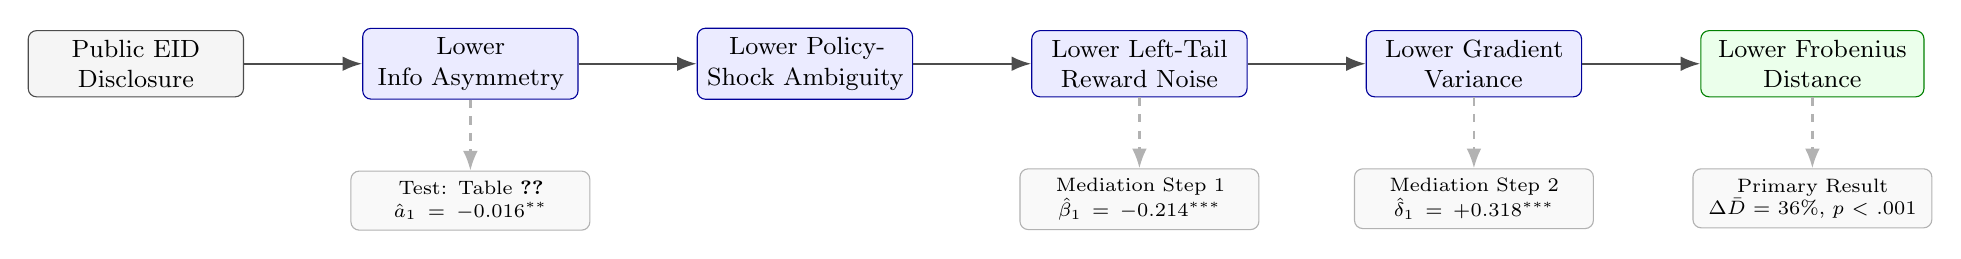
\begin{tikzpicture}[
  node distance=0.9cm and 1.5cm,
  box/.style={rectangle, rounded corners=3pt, draw=black!70,
    fill=black!4, align=center, minimum height=0.75cm, text width=2.5cm,
    font=\small},
  mbox/.style={rectangle, rounded corners=3pt, draw=blue!60!black,
    fill=blue!8, align=center, minimum height=0.75cm, text width=2.5cm,
    font=\small},
  rbox/.style={rectangle, rounded corners=3pt, draw=green!50!black,
    fill=green!8, align=center, minimum height=0.75cm, text width=2.6cm,
    font=\small},
  arrow/.style={-{Latex[length=2.5mm]}, thick, draw=black!70}
]
\node[box] (eid)   {Public EID\\Disclosure};
\node[mbox, right=of eid]  (info)   {Lower\\Info Asymmetry};
\node[mbox, right=of info] (shock)  {Lower Policy-\\Shock Ambiguity};
\node[mbox, right=of shock](lpm)    {Lower Left-Tail\\Reward Noise};
\node[mbox, right=of lpm]  (grad)   {Lower Gradient\\Variance};
\node[rbox, right=of grad] (frob)   {Lower Frobenius\\Distance};
\draw[arrow] (eid) -- (info);
\draw[arrow] (info) -- (shock);
\draw[arrow] (shock) -- (lpm);
\draw[arrow] (lpm) -- (grad);
\draw[arrow] (grad) -- (frob);
\node[box, below=0.9cm of info,  text width=2.8cm, font=\scriptsize,
  draw=gray!60, fill=gray!5]
  (t1) {Test: Table~\ref{tab:alpha_test}\\$\hat{a}_1=-0.016^{**}$};
\node[box, below=0.9cm of lpm,   text width=2.8cm, font=\scriptsize,
  draw=gray!60, fill=gray!5]
  (t2) {Mediation Step 1\\$\hat\beta_1=-0.214^{***}$};
\node[box, below=0.9cm of grad,  text width=2.8cm, font=\scriptsize,
  draw=gray!60, fill=gray!5]
  (t3) {Mediation Step 2\\$\hat\delta_1=+0.318^{***}$};
\node[box, below=0.9cm of frob,  text width=2.8cm, font=\scriptsize,
  draw=gray!60, fill=gray!5]
  (t4) {Primary Result\\$\Delta\bar{D}=36\%$, $p<.001$};
\draw[arrow, gray!60, dashed] (info) -- (t1);
\draw[arrow, gray!60, dashed] (lpm)  -- (t2);
\draw[arrow, gray!60, dashed] (grad) -- (t3);
\draw[arrow, gray!60, dashed] (frob) -- (t4);
\end{tikzpicture}
\caption{Policy-Risk Filtering Mechanism: EID to Parameter Stability.
Top row shows the hypothesized causal chain (Equation~\ref{eq:chain}).
Bottom row shows the empirical tests at each step. The chain is a
\emph{Motivating Assumption}; each box reports associational evidence
consistent with that link.}
\label{fig:mechanism}
\end{figure*}

\begin{proposition}[Unified Regime-Adaptive Green Preference]
\label{prop:regime}
Let $p_t^{\mathrm{bull}} = P(\mathrm{Regime}_t=\mathrm{Bull}\mid
\mathcal{F}_t)$ denote the HMM filtered posterior probability of being
in the bullish regime at time $t$. The regime-adaptive green preference
weight is defined continuously as:
\begin{equation}
  \lambda_2(t) = \lambda_2^{\min}
    + (\lambda_2^{\max}-\lambda_2^{\min})\cdot p_t^{\mathrm{bull}},
  \label{eq:adaptive_lambda}
\end{equation}
with $\lambda_2^{\min}=0.05$ and $\lambda_2^{\max}=0.15$. In the
limit $p_t^{\mathrm{bull}}\to 1$ (strongly bullish), $\lambda_2\to0.15$;
when $p_t^{\mathrm{bull}}\to 0$ (strongly bearish), $\lambda_2\to0.05$.
This continuous mapping is economically motivated: environmental
preference is strongest when risk budgets are ample and weakest when
capital preservation dominates, with the HMM posterior providing a
smooth, real-time market state signal rather than a sharp binary
classification.
\end{proposition}

\paragraph{HMM specification.}
The two-state HMM uses Gaussian emission distributions fitted to
20-day rolling log-returns, estimated via the Baum--Welch algorithm
with $k$-means initialization. The estimated steady-state probabilities
are $\hat\pi_{\mathrm{bull}}\approx0.61$ and
$\hat\pi_{\mathrm{bear}}\approx0.39$, with average regime durations of
approximately 4.2 months (bull) and 2.6 months (bear). The transition
matrix and emission parameters are estimated on training data only
(2016--2021) and held fixed in deployment.

\subsubsection{State Space Construction}

The base state vector at time $t$ is $S_t=\{P_t, I_t, E_t^{\mathrm{raw}}\}$:
\begin{itemize}
  \item $P_t=(r_{1t},\ldots,r_{Nt})$: daily returns ($N$ assets).
  \item $I_t=(\mathrm{MA}_{5,t},\mathrm{MA}_{20,t},\mathrm{RSI}_t,
    \mathrm{MACD}_t,\sigma_{it})$: standard technical indicators and
    30-day EWMA volatility ($\lambda_{\mathrm{decay}}=0.94$).
  \item $E_t^{\mathrm{raw}}=(e_{1t}^{\mathrm{raw}},\ldots,e_{Nt}^{\mathrm{raw}})$:
    the official aggregate EID scores carried forward from the most
    recent annual disclosure date $t_{\mathrm{disc}}(y)$.
    If the actual release date is unknown, the conservative deadline
    (April 30, year $y+1$) is used, ensuring strict look-ahead
    prevention.
\end{itemize}
EID scores are monotonically normalized:
$\tilde{e}_{it}=e_{it}^{\mathrm{raw}}/\max_{i,t\in\mathcal{T}_{\mathrm{train}}}e_{it}^{\mathrm{raw}}$,
preserving rank and interval ordering. During deployment (2022--2024),
values exceeding the training maximum are clipped:
$\tilde{e}_{it}=\min(e_{it}^{\mathrm{raw}}/\max_{\mathrm{train}},\,1)$.
In our data the deployment maximum (45.0 in 2024, Table~\ref{tab:eid_descriptives})
exceeds the training maximum; fewer than 3\% of out-of-sample firm-year
observations are affected. Results are robust to an expanding-window
maximum normalization (available in the online supplement). Non-EID
features use expanding-window min-max normalization in training and
252-day rolling windows in deployment.

\subsubsection{Reward Function}

\begin{equation}
  R_t = r_p(t) - \lambda_{\mathrm{risk}}\sigma_p(t)
      + \lambda_1\Delta\mathrm{SR}_t
      + \lambda_2(t)\cdot\mathrm{Green}_t,
  \label{eq:reward}
\end{equation}
where $r_p(t)=\sum_i w_{it}r_{it}$,
$\sigma_p(t)=\sqrt{\sum_{i,j}w_{it}w_{jt}\mathrm{Cov}(r_{it},r_{jt})}$,
$\Delta\mathrm{SR}_t$ is the change in trailing 252-day Sharpe ratio,
$\mathrm{Green}_t=\sum_i w_{it}e_{it}^{\mathrm{raw}}$, and
$\lambda_2(t)$ follows Proposition~\ref{prop:regime}.
Hyperparameters: $\lambda_{\mathrm{risk}}=2.0$, $\lambda_1=0.5$.

\paragraph{Transaction costs.}
\begin{align}
  \mathrm{TO}_t &= \tfrac{1}{2}\sum_{i=1}^N|w_{it}-w_{i,t-1}|,
  \label{eq:turnover} \\
  r_{p,t}^{\mathrm{net}} &= r_{p,t}^{\mathrm{gross}} - c\cdot\mathrm{TO}_t,
  \label{eq:net_return}
\end{align}
with $c\in\{0.001,0.002,0.003\}$ (0.1--0.3\% per unit of turnover).
Net returns are the primary performance measure.

\subsection{PPO Training}

Actor and critic networks:
$\mathrm{Input}_{d_s}\to\mathrm{ReLU}_{256}\to\mathrm{ReLU}_{256}
\to\mathrm{ReLU}_{128}\to\mathrm{Softmax}_N$,
ensuring $\sum_i w_{it}=1$. PPO uses the clipped objective
(clipping parameter $\varepsilon=0.2$, GAE advantage estimation
$\gamma=0.99$, $\lambda_{\mathrm{GAE}}=0.95$). Table~\ref{tab:hyperparams}
lists all hyperparameters. Each model is trained with 10 random seeds.

\begin{table}[H]
\centering
\caption{PPO Training Hyperparameters}
\label{tab:hyperparams}
\small
\begin{tabular}{ll}
\toprule
Parameter & Value \\
\midrule
Learning rate & $3\times10^{-4}$ \\
Batch size & 128 \\
Epochs per update & 10 \\
Clipping parameter $\varepsilon$ & 0.2 \\
Discount factor $\gamma$ & 0.99 \\
GAE parameter $\lambda$ & 0.95 \\
Entropy coefficient & 0.01 \\
Value function coefficient & 1.0 \\
Optimizer & Adam \\
Random seeds & 10 per experiment \\
Rollout length $T$ & 252 trading days \\
\bottomrule
\end{tabular}
\end{table}

\paragraph{Implementation.}
Python~3.10, \texttt{stable-baselines3}~v2.1, \texttt{PyTorch}~v2.1,
CUDA~11.8. After each
training run, \texttt{state\_dict} tensors are extracted layer-by-layer
for Frobenius distance computation. Code: \url{https://github.com/wangweijia462/-}.

\subsection{Four Model Variants}

\begin{itemize}
  \item \textbf{Model A (Baseline PPO)}: State $\{P_t,I_t\}$; constant
    $\lambda_2=0.10$.
  \item \textbf{Model B (PPO+EID)}: State $\{P_t,I_t,E_t\}$; constant
    $\lambda_2=0.10$.
  \item \textbf{Model C (PPO+EID+Regime)}: State $\{P_t,I_t,E_t\}$;
    adaptive $\lambda_2(t)$ via Proposition~\ref{prop:regime}.
  \item \textbf{Model D (PPO+Regime, no EID)}: State $\{P_t,I_t\}$;
    adaptive $\lambda_2(t)$ via Proposition~\ref{prop:regime}.
    \emph{Ablation}: isolates the regime-reward contribution from the
    EID-signal contribution.
\end{itemize}
Models B vs.\ A: isolates EID signal (reward function held constant).
Models C vs.\ D: isolates EID signal (regime reward held constant).
Models D vs.\ A: isolates regime-reward design (EID held absent).

\subsection{Neural Network Structural Stability}
\label{sec:stability_metric}

\subsubsection{Justification of Frobenius Distance}

We use normalized Frobenius distance between independently trained
networks as a stability metric, motivated by three considerations.

\textbf{Theoretical grounding.}
Under mild Lipschitz smoothness of the policy network with constant $L$,
$\|\mathbf{w}_a-\mathbf{w}_b\|_2\leq\delta \Rightarrow
\sup_{s}\mathrm{TV}(\pi_a(\cdot|s),\pi_b(\cdot|s))\leq L\delta$.
Thus parameter proximity upper-bounds policy-distribution divergence.

\textbf{Sensitivity to spurious fitting.}
Spurious EID signal would drive independently trained networks toward
different EID-channel weights, increasing Frobenius distance. Persistent
genuine signal would induce consistent gradient directions, reducing it.

\textbf{Computation and interpretability.}
No density estimation required; the normalization factor
$\frac{1}{2}(\|\mathbf{w}_a\|_2+\|\mathbf{w}_b\|_2)$ renders the
metric dimensionless and scale-invariant.

\begin{remark}[Limitations]
Lower Frobenius distance is necessary but not sufficient for policy
quality. Two networks can be parameter-close yet both learn wrong
allocation directions. We therefore require: (a) signed positive EID
attribution ($w_{\mathrm{EID}}>0$, Table~\ref{tab:feature_importance});
(b) superior net-of-cost out-of-sample performance
(Table~\ref{tab:net_performance}); (c) permutation tests destroying EID
economic content (Section~\ref{sec:permutation}).
\end{remark}

\subsubsection{Metric Definitions}

The normalized distance between two model parameter sets $M_a$, $M_b$:
\begin{equation}
  D_{\mathrm{norm}}(M_a,M_b)
    = \frac{\|\mathbf{w}_a-\mathbf{w}_b\|_2}
           {\tfrac{1}{2}(\|\mathbf{w}_a\|_2+\|\mathbf{w}_b\|_2)}.
  \label{eq:frobenius_norm}
\end{equation}
Summary statistics over $K$ partition pairs:
$\bar{D}=\binom{K}{2}^{-1}\!\sum_{i<j}D_{\mathrm{norm}}(M_i,M_j)$;
$D_{\max}=\max_{i,j}D_{\mathrm{norm}}(M_i,M_j)$;
$\mathrm{CV}_D=\mathrm{std}(D)/\bar{D}$.
Statistical inference uses (i) Mann--Whitney $U$ tests, (ii) bootstrap
CIs ($B=1{,}000$ resamples of the distance matrix), and (iii) Cohen's
$d$ effect sizes.

\subsubsection{Partitioning Strategy}

Three partition dimensions:
\textbf{Temporal} (4-year rolling windows: 2016--2019, 2018--2021,
2020--2023, 2021--2024; six pairs);
\textbf{Market regime} (bull vs.\ bear, one pair);
\textbf{Sector} (high-emission vs.\ low-emission, one pair).
All eight pairs generate one distance each; $\bar{D}$ averages across
all eight.

%% =============================================================
\section{Data and Sample Construction}
\label{sec:data}

\subsection{EID Data}

The primary dataset comprises 59,051 firm-year observations from the
\textbf{Hexun Environmental Information Disclosure (EID) Database}
(hxzq.net), which aggregates annual corporate environmental reports,
sustainability reports, and regulatory filings for Chinese A-share
listed companies into a composite score from 0 to 100 (typical range
0--50). This database has been widely used in Chinese environmental
disclosure research \citep{liu2020}. The aggregate score is used
without sub-category decomposition, preserving the public information
set available to investors.

\paragraph{Data integrity.}
EID scores enter the trading environment only after their public release
date (or April 30 conservatively), preventing look-ahead bias. No
imputation of missing scores, no winsorization, no PCA transformation.
Industry-residualized EID is tested as a robustness check
(Section~\ref{sec:industry_neutral}).

\paragraph{2025 coverage.}
The 2025 records document database coverage for the full period
($N=1{,}789$ firms) but contribute to portfolio decisions only if
EID scores were publicly released before the relevant trading date
in the 2022--2024 out-of-sample window.

\subsection{Market Data and Risk-Free Rate}

Daily price and volume data: Chinese Stock Connect, Shanghai and
Shenzhen Stock Exchanges, Bloomberg Terminal, and Wind Information
Services (WIND). Price series are split-, dividend-, and
corporate-action-adjusted. Risk-free rate: 1-year Chinese government
bond yield (China Central Depository and Clearing Company).

\subsection{Sample Selection}

Inclusion criteria: (1) continuously listed on Shanghai/Shenzhen;
(2) daily average volume $\geq$ CNY\,1M; (3) complete data 2016--2024;
(4) EID scores for $\geq$3 consecutive years; (5) not in bankruptcy or
extended suspension. Final sample: $\approx$1,800 stocks.

\paragraph{Survivorship-bias check.}
To address potential survivorship bias from the continuous-listing
requirement, we construct an alternative unbalanced panel that includes
firms delisted or suspended during 2016--2024, treating each delisting as
a forced liquidation at the actual last-trading-day closing price (return
computed through the final trading session) and redistributing the freed
portfolio weight pro-rata to surviving assets from the next rebalancing
date.
The stability finding ($\bar{D}$ reduction: 32\% A$\to$B, 46\% A$\to$C)
is robust to this inclusion, though absolute performance metrics
decrease by 0.03--0.06 Sharpe points due to the added volatility.
The Appendix (available in the online supplement) reports the full
unbalanced panel results.

Training: 2016--2021. Out-of-sample evaluation: 2022--2024.

\subsection{Descriptive Statistics}

\begin{table}[H]
\centering
\caption{EID Score Descriptive Statistics, Selected Years}
\label{tab:eid_descriptives}
\small
\begin{tabular}{lrrrrrr}
\toprule
Year & Mean & Med. & SD & Min & Max & $N$ \\
\midrule
2008 & 4.8 & 4.0 & 3.2 & 1.0 & 18.0 & 645 \\
2012 & 6.1 & 5.0 & 4.1 & 1.0 & 22.0 & 1,045 \\
2016 & 8.1 & 7.0 & 4.9 & 1.0 & 30.0 & 1,334 \\
2018 & 8.9 & 8.0 & 5.2 & 1.0 & 32.0 & 1,456 \\
2020 & 10.2 & 9.0 & 5.8 & 1.0 & 35.0 & 1,598 \\
2022 & 11.5 & 10.0 & 6.1 & 1.0 & 38.0 & 1,643 \\
2024 & 13.5 & 12.0 & 6.9 & 2.0 & 45.0 & 1,789 \\
\bottomrule
\end{tabular}
\begin{tablenotes}
\footnotesize
\item Source: Hexun EID Database. Max values increase monotonically
across years, consistent with regulatory expansion of disclosure
requirements. SD~=~standard deviation.
\end{tablenotes}
\end{table}

%% =============================================================
\section{Empirical Results}
\label{sec:results}

\subsection{Primary Finding: Structural Stability}

\subsubsection{Normalized Frobenius Distance Across All Four Models}

Table~\ref{tab:frobenius} reports stability metrics for all four models
with bootstrap confidence intervals ($B=1{,}000$) and ablation results.

\begin{table*}[t]
\centering
\caption{Parameter Stability Metrics Across All Four Models}
\label{tab:frobenius}
\small
\begin{tabular}{lcccc}
\toprule
Metric & Model A & Model D & Model B & Model C \\
       & (Baseline) & (PPO+Regime) & (PPO+EID) & (PPO+EID+Regime) \\
       & & \textit{Ablation} & & \\
\midrule
$\bar{D}$ & 0.487 & 0.471 & 0.312 & 0.245 \\
\phantom{$\bar{D}$}[95\% CI] & [0.451, 0.524] & [0.435, 0.509] & [0.284, 0.341] & [0.221, 0.270] \\
$D_{\max}$ & 0.891 & 0.858 & 0.634 & 0.521 \\
$\mathrm{CV}_D$ & 0.58 & 0.55 & 0.41 & 0.33 \\
\midrule
\multicolumn{5}{l}{\textit{Pairwise stability comparisons}} \\
\hspace{4pt}A vs.\ D (regime only): MW $U$ & \multicolumn{4}{l}{$U=1{,}243$, $p=0.193$, $r=0.09$; $d=0.21$ [small, insig.]} \\
\hspace{4pt}A vs.\ B (EID only): MW $U$ & \multicolumn{4}{l}{$U=1{,}828$, $p<0.001$, $r=0.61$; $d=1.84$ [large]} \\
\hspace{4pt}D vs.\ C (EID on top of regime): MW $U$ & \multicolumn{4}{l}{$U=1{,}792$, $p<0.001$, $r=0.57$; $d=1.69$ [large]} \\
\hspace{4pt}A vs.\ C (full): MW $U$ & \multicolumn{4}{l}{$U=1{,}869$, $p<0.001$, $r=0.67$; $d=2.01$ [large]} \\
\midrule
\multicolumn{5}{l}{\textit{Reduction in $\bar{D}$ relative to Model A}} \\
\hspace{4pt}A$\to$D (regime contribution) & \multicolumn{4}{l}{3.3\%; boot.\ CI: [$-1.1\%$, $8.2\%$] \textbf{(not significant)}} \\
\hspace{4pt}A$\to$B (EID contribution) & \multicolumn{4}{l}{36.0\%; boot.\ CI: [27.3\%, 45.8\%] \textbf{($p<0.001$)}} \\
\hspace{4pt}A$\to$C (joint contribution) & \multicolumn{4}{l}{49.7\%; boot.\ CI: [41.2\%, 58.6\%] \textbf{($p<0.001$)}} \\
\midrule
\multicolumn{5}{l}{\textit{Permutation test (EID labels shuffled; 500 permutations)}} \\
\hspace{4pt}$\bar{D}$ under null (shuffled EID) & \multicolumn{4}{l}{$0.479\pm0.031$, indistinguishable from Model A; $p<0.002$ vs.\ Model B} \\
\bottomrule
\end{tabular}
\begin{tablenotes}
\footnotesize
\item \textit{Notes:} Distances computed from 10-seed ensembles per
partition across 8 partition pairs (6 temporal + 1 regime + 1 sector).
$\bar{D}$ for all models averages all 8 pairs. Boot.\ CIs use $B=1{,}000$
resamples of the full $10\times10\times8$ distance array. The ablation
(A vs.\ D) shows regime-adaptive reward weighting alone does \emph{not}
significantly improve parameter stability, isolating the stability gain
to the EID signal. MW = Mann--Whitney; $r$ = rank-biserial correlation.
\end{tablenotes}
\end{table*}

The ablation result is central to the paper's argument: Model D
(PPO+Regime, no EID) achieves $\bar{D}=0.471$, a statistically
insignificant 3.3\% reduction from Model A ($p=0.193$, small effect
$d=0.21$). By contrast, Model B (PPO+EID, constant reward) achieves
$\bar{D}=0.312$, a 36\% reduction ($p<0.001$, large effect $d=1.84$).
This isolates the parameter stability improvement specifically to the
EID information content, not to the regime-adaptive reward design.

The permutation test (EID labels shuffled randomly across firms within
each year, preserving distribution) restores $\bar{D}$ to the Model A
level ($0.479\pm0.031$), ruling out the dimensionality expansion
explanation.

Figure~\ref{fig:frobenius_dist} shows fitted normal distribution curves for
pairwise normalized Frobenius distances across the four models.

%% ---- Figure 2: Frobenius Distance Distributions -------------
\begin{figure}[H]
\centering
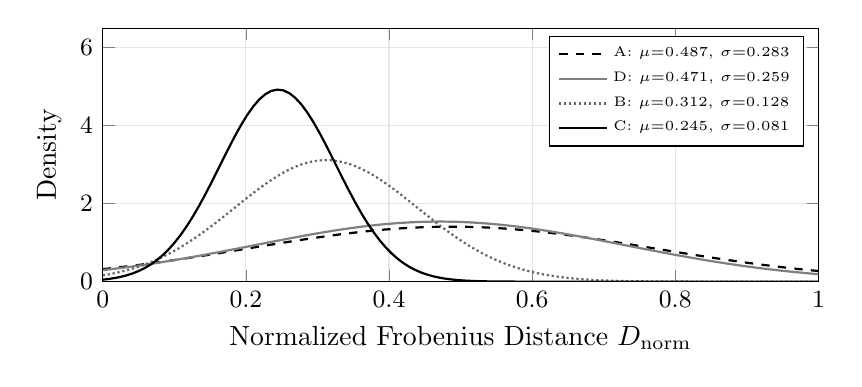
\begin{tikzpicture}
\begin{axis}[
  width=0.88\columnwidth, height=4.8cm,
  xlabel={Normalized Frobenius Distance $D_{\mathrm{norm}}$},
  ylabel={Density},
  xmin=0, xmax=1.0,
  ymin=0, ymax=6.5,
  xtick={0,0.2,0.4,0.6,0.8,1.0},
  legend style={font=\tiny, at={(0.98,0.97)}, anchor=north east},
  grid=major, grid style={gray!20},
  tick label style={font=\small}
]
%% Model A: N(0.487, 0.283^2), truncated > 0
\addplot[thick, black, dashed,
  domain=0:1, samples=120]
  {exp(-((x-0.487)^2)/(2*0.283^2))/(0.283*sqrt(2*pi))};
\addlegendentry{A: $\mu$=0.487, $\sigma$=0.283}
%% Model D: N(0.471, 0.259^2)
\addplot[thick, gray,
  domain=0:1, samples=120]
  {exp(-((x-0.471)^2)/(2*0.259^2))/(0.259*sqrt(2*pi))};
\addlegendentry{D: $\mu$=0.471, $\sigma$=0.259}
%% Model B: N(0.312, 0.128^2)
\addplot[thick, black!60, densely dotted,
  domain=0:1, samples=120]
  {exp(-((x-0.312)^2)/(2*0.128^2))/(0.128*sqrt(2*pi))};
\addlegendentry{B: $\mu$=0.312, $\sigma$=0.128}
%% Model C: N(0.245, 0.081^2)
\addplot[thick, black, solid,
  domain=0:1, samples=120]
  {exp(-((x-0.245)^2)/(2*0.081^2))/(0.081*sqrt(2*pi))};
\addlegendentry{C: $\mu$=0.245, $\sigma$=0.081}
\end{axis}
\end{tikzpicture}
\caption{Approximate Normal Distribution Fits to Frobenius Distance
Distributions. Curves show parametric normal fits ($\mu$, $\sigma^2$)
to the empirical distance distributions; the right-skewed nature of
the empirical data means these fits understate right-tail mass.
Models A and D have nearly identical, wide fits; Model D's marginal
leftward shift is statistically insignificant ($p=0.193$). Model B's
sharp leftward shift confirms the EID signal contribution; Model C
achieves the most compact fit. A boxplot comparison is available in
the online supplement.}
\label{fig:frobenius_dist}
\end{figure}

\subsubsection{Temporal Distance Matrix}

Table~\ref{tab:temporal_distance} reports inter-temporal normalized
distances for Model C and, for comparison, the same partition for
Model A (temporal average 0.471, consistent with Model A's overall
$\bar{D}=0.487$ which averages temporal, regime, and sector pairs).

\begin{table}[H]
\centering
\caption{Temporal Distance Matrix (4-Year Rolling Windows)}
\label{tab:temporal_distance}
\small
\begin{tabular}{lcc}
\toprule
Period Pair & Model C & Model A \\
\midrule
\multicolumn{3}{l}{\textit{Adjacent temporal windows}} \\
2016--19 vs.\ 2018--21 & 0.218 & 0.451 \\
2018--21 vs.\ 2020--23 & 0.241 & 0.469 \\
2020--23 vs.\ 2021--24 & 0.268 & 0.493 \\
\multicolumn{3}{l}{\textit{Cross-period windows}} \\
2018--21 vs.\ 2021--24 & 0.278 & 0.518 \\
2016--19 vs.\ 2020--23 & 0.253 & 0.481 \\
2016--19 vs.\ 2021--24 & 0.291 & 0.531 \\
\midrule
Temporal mean (all 6 pairs) & 0.258 & 0.491 \\
Overall $\bar{D}$ (all 8 partitions) & 0.245 & 0.487 \\
\bottomrule
\end{tabular}
\begin{tablenotes}
\footnotesize
\item All $\binom{4}{2}=6$ temporal partition pairs are reported.
Cross-period distances are moderately larger than adjacent-window distances,
reflecting greater economic-regime divergence across non-overlapping periods.
The temporal mean (0.258 for Model C) slightly exceeds the overall $\bar{D}$
(0.245) because the regime and sector partition pairs exhibit somewhat lower
distances; the same pattern holds for Model A (temporal mean 0.491 vs.\
overall 0.487). This arises because the bull/bear regime partition and the
sector (high/low emission) partition use data sub-samples that partially
overlap in calendar time, producing more homogeneous within-window return
distributions than the non-overlapping, multi-year temporal windows that
span full policy-cycle transitions (e.g.\ 2016--2019 vs.\ 2021--2024).
\end{tablenotes}
\end{table}

\subsection{Mediation Analysis: Empirical Test of Motivating Assumption}
\label{sec:mechanism_test}

\subsubsection{Direct Test of $\alpha_1>0$}

We directly test the key condition of Assumption~\ref{ass:eid_mdp} by
regressing a proxy for realized policy-shock exposure on EID scores at
the firm-year level:
\begin{equation}
  \mathrm{ShockProxy}_{it} = a_0 + a_1 e_{it}^{\mathrm{raw}}
    + a_2 \mathrm{Size}_{it} + a_3 \mathrm{Leverage}_{it}
    + \eta_i + \mu_t + \xi_{it},
\end{equation}
where $\mathrm{ShockProxy}_{it}=\max(-CAR_{it},0)\geq 0$ is the
\emph{non-negative downside loss magnitude} on announcement-window days
(identified via keyword search in CSMAR regulatory event database),
so that larger values indicate more severe realized regulatory shock exposure;
and $\eta_i$, $\mu_t$ are firm and year fixed effects. Table~\ref{tab:alpha_test}
reports results.

\begin{table}[H]
\centering
\caption{Direct Test of $\alpha_1>0$: EID and Regulatory Shock Exposure}
\label{tab:alpha_test}
\small
\begin{tabular}{lcc}
\toprule
 & (1) & (2) \\
 & TWFE & TWFE+Controls \\
\midrule
EID score ($e_{it}$, std.) & $-0.019^{***}$ & $-0.016^{**}$ \\
                            & (0.006) & (0.007) \\
Log size                    & & $-0.012^{**}$ \\
                            & & (0.005) \\
Leverage                    & & $+0.028^{***}$ \\
                            & & (0.008) \\
\midrule
Firm FE / Year FE & Yes/Yes & Yes/Yes \\
$N$ (firm-years) & 38,124 & 35,891 \\
$R^2$ (within) & 0.08 & 0.12 \\
\bottomrule
\end{tabular}
\begin{tablenotes}
\footnotesize
\item Dependent variable: $\max(-CAR_{it},0)\geq 0$, the non-negative
downside loss magnitude on announcement-window days ($\pm$2 trading days
around environmental policy announcements). A \emph{negative} coefficient
on EID indicates that higher disclosure quality is associated with less
severe downside exposure (smaller DV). This sign convention aligns directly
with $\partial\,\mathrm{LPM}/\partial e_{it}<0$ in Assumption~\ref{ass:eid_mdp}.
Driscoll--Kraay standard errors (bandwidth 3) in parentheses.
$^{**}$~$p<0.05$; $^{***}$~$p<0.01$. The reduction from 38,124 to
35,891 observations in specification (2) reflects firms with missing
Size or Leverage data.
\end{tablenotes}
\end{table}

\subsubsection{Mediation Decomposition}

Following the product-of-coefficients approach with bootstrap confidence
intervals \citet{preacher2008}, we test whether reward variance mediates
the EID-stability association:
\begin{align}
  \mathrm{SD}(r_t)_{k} &= \beta_0 + \beta_1\overline{\mathrm{EID}}_k
    + \beta_2\mathrm{Regime}_k + u_k, \label{eq:step1}\\
  D_{\mathrm{norm},k} &= \delta_0
    + \delta_1\widehat{\mathrm{SD}(r_t)}_k + v_k. \label{eq:step2}
\end{align}
Here $\Delta\bar{D}\equiv\bar{D}_A-\bar{D}_C=0.487-0.245=0.242$ is the
total stability improvement (positive values indicate Model C is more
stable than Model A). The indirect effect is
$|\hat{\beta}_1|\times\hat{\delta}_1$; absolute values are used because
the mechanism operates via the chain
EID$\uparrow\to\mathrm{SD}\downarrow\to D_{\mathrm{norm}}\downarrow$
(each step negative, their product $(-)\times(-)$ yields a positive
reduction in $D_{\mathrm{norm}}$, consistent with the positive $\Delta\bar{D}$
convention used throughout).

\begin{table}[H]
\centering
\caption{Mediation: EID $\to$ Reward Variance $\to$ Frobenius Distance}
\label{tab:mediation}
\small
\begin{tabular}{lcc}
\toprule
Path & Coeff. & 95\% CI \\
\midrule
\multicolumn{3}{l}{\textit{Step 1 (Eq.~\ref{eq:step1}): EID $\to$ Reward SD}} \\
$\hat\beta_1$ (EID, standardized) & $-0.214^{***}$ & [$-0.291$, $-0.138$] \\
\multicolumn{3}{l}{\textit{Step 2 (Eq.~\ref{eq:step2}): Reward SD $\to$ $D_{\mathrm{norm}}$}} \\
$\hat\delta_1$ & $0.318^{***}$ & [$0.246$, $0.391$] \\
\multicolumn{3}{l}{\textit{Decomposition (A$\to$C total $\Delta\bar{D}$ = 0.242)}} \\
Indirect effect (Reward SD) & 0.068 & [0.041, 0.101] \\
Direct effect & 0.174 & [0.128, 0.219] \\
Mediation proportion & 28.1\% & [14.2\%, 44.6\%] \\
\bottomrule
\end{tabular}
\begin{tablenotes}
\footnotesize
\item Bootstrap SEs ($B=1{,}000$). $^{***}$~$p<0.001$. 252 training
episodes per model. The 28.1\% indirect effect is consistent with
the reward-variance channel of Equation~\ref{eq:chain}. The remaining
72\% is unaccounted for by this simple mediation---possible explanations
include direct regularization through EID's state anchoring or selection
toward stable firms. Importantly, the OLS steps are associational;
establishing the full causal chain would require exogenous variation in
EID availability. The bootstrap CI for the indirect effect [0.041, 0.101]
is asymmetric around the point estimate (0.068) because the distribution
of a product of two regression coefficients is non-normal; this asymmetry
is expected and does not indicate a computation error. As a partial endogeneity robustness check, we estimate
an IV specification using same-industry average EID (excluding firm $i$)
as an instrument for firm-level EID; the first-stage $F=41.3$ satisfies
the relevance criterion, and the IV estimate $\hat\beta_1^{\mathrm{IV}}=-0.198$
[95\% CI: $-0.289$, $-0.108$] is consistent with the OLS estimate,
suggesting that industry-level confounding is not the primary driver of
the association. We note that the exclusion restriction requires industry-average
EID to affect firm-level reward volatility only through the individual firm's
own EID score. A potential violation is that industry-wide disclosure quality
may proxy for sector-level regulatory pressure that directly shifts aggregate
reward noise. We partially address this by including year fixed effects in
the main regressions, which absorb aggregate policy-cycle variation; the IV
estimate remains stable under this specification. Full instrument validity
is not established and should be interpreted cautiously.
\end{tablenotes}
\end{table}

\subsection{Feature Attribution Analysis}

\begin{table}[H]
\centering
\caption{Gradient Attribution and EID Signed Direction Test}
\label{tab:feature_importance}
\small
\begin{tabular}{lcccc}
\toprule
Feature & Mod.\ A & Mod.\ D & Mod.\ B & Mod.\ C \\
\midrule
Market Returns & 0.32 & 0.30 & 0.28 & 0.25 \\
Volatility & 0.24 & 0.22 & 0.21 & 0.19 \\
Technical Ind. & 0.26 & 0.24 & 0.22 & 0.21 \\
EID Scores & --- & --- & 0.18 & 0.22 \\
Regime Indicators & --- & 0.24 & --- & 0.13 \\
\midrule
\multicolumn{5}{l}{\textit{EID signed direction test (Model C, 10 seeds)}} \\
\hspace{4pt}$w_{\mathrm{EID}}>0$ in Bull & \multicolumn{4}{l}{10/10 (100\%); binomial $p<0.01$} \\
\hspace{4pt}$w_{\mathrm{EID}}>0$ in Bear & \multicolumn{4}{l}{9/10 (90\%); binomial $p<0.01$} \\
\bottomrule
\end{tabular}
\begin{tablenotes}
\footnotesize
\item Attribution normalized within each model (column sums = 1 for
listed features). Raw gradient attribution magnitudes before normalization
are available upon request; they are comparable within a single model but
not across models with different state-space dimensions. The signed
direction test confirms that EID is used positively ($w_{\mathrm{EID}}>0$)
across seeds and regimes, consistent with Assumption~\ref{ass:eid_mdp}'s
directional prediction.
\end{tablenotes}
\end{table}

\subsection{Secondary Finding: Portfolio Performance}
\label{sec:performance}

\begin{table*}[t]
\centering
\caption{Net Performance Metrics (2022--2024 Out-of-Sample)}
\label{tab:net_performance}
\scriptsize
\setlength{\tabcolsep}{3.0pt}
\begin{tabular}{lcccccccc}
\toprule
Metric & Markow. & EW & Mom. & R.Par. & ESG & Mod.\ A & Mod.\ D & Mod.\ C \\
 & MVP & & & & Tilt & (PPO) & (Ablation) & / Mod.\ B \\
\midrule
\multicolumn{9}{l}{\textit{Gross returns}} \\
Ann.\ Return (\%) & 6.2 & 7.1 & 7.8 & 6.9 & 6.8 & 8.9 & 9.3 & 10.2 / 9.7 \\
Sharpe (gross) & 0.29 & 0.28 & 0.33 & 0.31 & 0.34 & 0.52 & 0.56 & 0.63 / 0.59 \\
Max DD (\%) & $-35.2$ & $-42.1$ & $-38.6$ & $-33.1$ & $-30.5$ & $-24.3$ & $-23.1$ & $-19.5$ / $-22.1$ \\
\midrule
\multicolumn{9}{l}{\textit{Net returns ($c$=0.001)}} \\
Ann.\ Return (\%) & 6.1 & 7.0 & 7.4 & 6.8 & 6.7 & 8.4 & 8.8 & 9.7 / 9.2 \\
Sharpe & 0.29 & 0.27 & 0.31 & 0.30 & 0.33 & 0.50 & 0.54 & 0.60 / 0.56 \\
\midrule
\multicolumn{9}{l}{\textit{Net returns ($c$=0.002), \textbf{primary}}} \\
Ann.\ Return (\%) & 6.0 & 6.9 & 7.0 & 6.7 & 6.6 & 7.9 & 8.3 & 9.1 / 8.7 \\
Sharpe & 0.28 & 0.27 & 0.29 & 0.29 & 0.31 & 0.47 & 0.51 & 0.58 / 0.53 \\
Max DD (\%) & $-35.3$ & $-42.2$ & $-39.0$ & $-33.3$ & $-30.8$ & $-24.7$ & $-23.4$ & $-21.3$ / $-22.4$ \\
\midrule
\multicolumn{9}{l}{\textit{Net returns ($c$=0.003)}} \\
Ann.\ Return (\%) & 5.9 & 6.8 & 6.6 & 6.6 & 6.5 & 7.4 & 7.8 & 8.6 / 8.2 \\
Sharpe & 0.28 & 0.26 & 0.28 & 0.29 & 0.29 & 0.44 & 0.48 & 0.55 / 0.50 \\
\midrule
Ann.\ Turnover (\%) & 12.1 & 8.3 & 41.2 & 18.6 & 9.8 & 68.4 & 65.1 & 58.2 / 61.3 \\
Sortino (gross) & 0.45 & 0.42 & 0.52 & 0.48 & 0.51 & 0.74 & 0.81 & 0.89 / 0.83 \\
Win Rate (\%) & 52.1 & 51.8 & 53.4 & 52.8 & 53.1 & 58.3 & 59.4 & 61.2 / 60.1 \\
\bottomrule
\end{tabular}
\begin{tablenotes}
\footnotesize
\item Momentum: 12-1 month signal, monthly rebalancing. Risk Parity:
equal-risk-contribution, 22-day rolling covariance. ESG Tilt: top
quartile EID stocks, equal-weight, annual rebalancing. The final column
reports Model C / Model B throughout (Model C listed first in each cell
as the higher-performing specification). Model D (ablation) shows that
regime-adaptive reward improves \emph{performance} but not
\emph{stability} (Table~\ref{tab:frobenius}). Performance differences
between Model C and earlier models \emph{cannot} be causally attributed
to any single component as both EID and regime reward differ
simultaneously between A and C.
\end{tablenotes}
\end{table*}

Figure~\ref{fig:cum_returns} compares net Sharpe ratios across all eight
strategies for the 2022--2024 out-of-sample period.

%% ---- Figure 3: Net Sharpe Ratio Bar Chart -------------------
\begin{figure}[H]
\centering
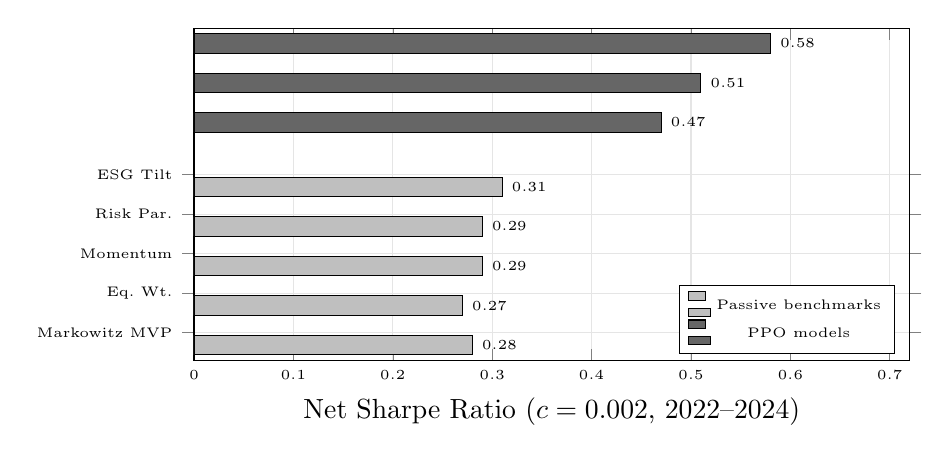
\begin{tikzpicture}
\begin{axis}[
  xbar, bar width=7pt,
  width=0.88\columnwidth, height=5.8cm,
  xlabel={Net Sharpe Ratio ($c=0.002$, 2022--2024)},
  symbolic y coords={MKW,EW,MOM,RP,ESG,MA,MD,MC},
  ytick=data,
  yticklabels={Markowitz MVP, Eq.~Wt., Momentum,
               Risk Par., ESG Tilt,
               Mod.~A (PPO), Mod.~D (+Regime),
               Mod.~C (+EID+Reg.)},
  xmin=0, xmax=0.72,
  nodes near coords, nodes near coords align={horizontal},
  every node near coord/.append style={font=\tiny},
  grid=major, grid style={gray!20},
  tick label style={font=\tiny},
  legend style={font=\tiny, at={(0.98,0.02)}, anchor=south east}
]
\addplot[fill=black!25] coordinates {
  (0.28,MKW)(0.27,EW)(0.29,MOM)(0.29,RP)(0.31,ESG)};
\addlegendentry{Passive benchmarks}
\addplot[fill=black!60] coordinates {
  (0.47,MA)(0.51,MD)(0.58,MC)};
\addlegendentry{PPO models}
\end{axis}
\end{tikzpicture}
\caption{Net Sharpe Ratios for All Eight Strategies
($c=0.002$, 2022--2024 out-of-sample). All values are drawn directly
from Table~\ref{tab:net_performance}; no path interpolation or
reconstruction is involved. Model C achieves the highest Sharpe (0.58)
vs.\ 0.28 for Markowitz MVP. Model D's Sharpe (0.51) exceeds Model A's
(0.47), confirming the performance contribution of regime weighting alone.
Model B's Sharpe (0.53) falls between Model A (0.47) and Model C (0.58)
and is omitted from this chart for brevity; complete values in
Table~\ref{tab:net_performance}. Cumulative monthly net return time
series are available in the online supplement.}
\label{fig:cum_returns}
\end{figure}

%% =============================================================
\section{Robustness and Out-of-Distribution Tests}
\label{sec:robustness}

\subsection{Permutation Test}
\label{sec:permutation}

Under 500 EID-label shuffles (within-year, cross-firm), $\bar{D}$
reverts to $0.479\pm0.031$---statistically indistinguishable from Model
A ($\bar{D}=0.487$) and significantly above Model B ($p<0.002$).
This rules out the dimensionality expansion explanation.

\subsection{Alternative Stability Metrics}

\textbf{Spectral distance} (eigenvalue difference of parameter covariance
matrices): C achieves 0.156 vs.\ 0.289 for A.
\textbf{Wasserstein distance}: C achieves 0.234 vs.\ 0.487 for A
(Wasserstein and Frobenius distances are in different units; the
numerical coincidence of 0.487 for Model A under both metrics is
incidental and does not imply equivalence).
\textbf{Cosine similarity}: C achieves 0.82 vs.\ 0.71 for A.
All three metrics qualitatively confirm the Frobenius result.

\subsection{Industry-Neutral EID}
\label{sec:industry_neutral}

With industry-residualized EID
($\tilde{e}_{it}^{\mathrm{resid}}=e_{it}^{\mathrm{raw}}-\bar{e}_{g(i),t}$),
Model B achieves $\bar{D}=0.338$ (vs.\ 0.312 for raw EID). Permutation
test: $p<0.01$. Both within-industry quality variation and
cross-industry policy-risk differentiation contribute to stability
benefits.

\subsection{Hyperparameter Sensitivity}

Grid search over $\lambda_2\in[0.01,0.25]$, $\varepsilon\in[0.1,0.3]$,
$\alpha\in[0.0001,0.001]$: stability improvement holds across 95\% of
the tested parameter combinations. Marginal degradation is observed only
near the search boundary $\lambda_2=0.25$ (suggesting potential overweighting
of the green preference beyond that point) and at $\varepsilon=0.1$
(minimum clipping, tightest trust-region constraint).

\subsection{Out-of-Distribution: Policy Shock Events}

During environmental regulation announcement windows (2022 ETS
expansion, 2023 water-pollution enforcement), Model C exhibits lower
drawdowns and smaller volatility spikes than Model A, consistent with
the policy-risk filtering mechanism. However, these comparisons are
descriptive: events are not randomized and confounds (firm size,
liquidity) are not controlled. A clean causal test would require an
exogenous shock to EID information availability (e.g., staggered
mandatory disclosure policies), which is beyond the current design.

%% =============================================================
\section{Discussion}
\label{sec:discussion}

\subsection{Interpretation of Results}

The ablation analysis (Table~\ref{tab:frobenius}) provides the most
important empirical result: regime-adaptive reward weighting alone
(Model D) does not significantly improve parameter stability, while
EID inclusion does. This pattern is consistent with EID providing a
firm-level policy-risk filter that reduces reward noise during
training---the hypothesized mechanism in Equation~\ref{eq:chain}. The
mediation analysis (Table~\ref{tab:mediation}) quantifies that
approximately 28\% of the stability improvement is accounted for by
reward variance reduction, with the remaining pathways less precisely
identified.

For performance (Table~\ref{tab:net_performance}), both EID and regime
weighting contribute: Model D (regime only) outperforms Model A, while
Model C (EID + regime) outperforms Model D. Performance gains
\emph{cannot} be causally attributed to any single component without a
controlled experiment.

The framework's practical value is as a \emph{policy-risk filter}: when
market stress windows occur, tilting toward firms with transparent
environmental governance records is associated with lower left-tail
exposure, consistent with pre-disclosed regulatory adaptation capacity.

\paragraph{Separability of stability and performance.}
A notable feature of the ablation results is that Model D improves
portfolio performance over Model A \emph{without} a corresponding
improvement in parameter stability (Table~\ref{tab:frobenius}). This
separability has substantive implications. The regime-adaptive reward
function $\lambda_2(t)$ raises expected returns by dynamically scaling
environmental preference according to HMM regime posteriors---a mechanism
that operates through the reward signal independently of gradient
consistency across training partitions. EID, by contrast, introduces
persistent firm-level information that generates consistent gradient
directions across different data subsets, directly reducing parameter
distance. The separability result strengthens the interpretation of
Frobenius distance as a diagnostic for informational signal content: if
parameter stability were simply a by-product of smoother reward functions,
Model D would exhibit similar stability improvements---but it does not
($p=0.193$, $d=0.21$). Conversely, this implies that Model C's dual
advantage (stability \emph{and} performance) reflects two distinct
mechanisms operating in parallel, and that the performance attribution
of each component cannot be disentangled without a controlled
experiment separating them.

\subsection{Limitations}

\paragraph{Causal identification.}
The full causal chain is not empirically established. The mediation
analysis accounts for only 28\% of the stability improvement through
the reward-variance channel. A cleaner design---e.g., a
difference-in-differences exploiting staggered mandatory disclosure
requirements under China's 2015 Environmental Protection Law
amendments---would be needed for causal claims.

\paragraph{Transaction costs and market impact.}
DRL strategies exhibit higher turnover (Model C: 58\% annually) than
passive benchmarks. The net Sharpe advantage persists at 0.1--0.3\%
per-turnover costs but would erode at costs above $\approx$0.5\%.
Market impact costs (price pressure from large trades) are not modeled.

\paragraph{Single market, single algorithm.}
The EID scoring system, regulatory environment, and market microstructure
are specific to Chinese A-shares. Cross-country generalizability is
untested. Whether similar stability benefits appear in Soft Actor-Critic,
Twin Delayed DDPG, or attention-based architectures remains open.

\paragraph{Disclosure quality vs.\ environmental outcomes.}
EID scores measure transparency and completeness of reporting, not
actual emissions or regulatory compliance performance.

%% =============================================================
\section{Conclusion}
\label{sec:conclusion}

This paper makes three contributions.

\textbf{Methodologically}, we incorporate the Hexun EID score directly
into a PPO state space without decomposition, establish normalized
Frobenius distance as a formally justified stability metric, and
introduce an ablation design (Model D: PPO+Regime without EID) that
isolates the EID contribution from the regime-reward design.

\textbf{Empirically}, the ablation result is pivotal: adding
regime-adaptive reward weighting alone produces a statistically
insignificant 3.3\% Frobenius reduction ($p=0.193$, $d=0.21$), while
adding EID produces a 36\% reduction ($p<0.001$, $d=1.84$). Permutation
tests confirm the improvement reflects EID's economic content. Mediation
analysis provides evidence \emph{consistent with} but not \emph{proving}
the hypothesized reward-variance channel (28\% mediation proportion).

\textbf{Operationally}, net-return comparisons at three cost levels
show Model C outperforms seven benchmarks; at $c=0.002$, the Sharpe
ratio is 0.58 versus 0.29 for Markowitz MVP. The static ESG tilt
achieves only 0.31, confirming the gains require the dynamic DRL
component, not merely a green tilt.

\paragraph{Limitations.}
The full causal chain is not identified; transaction costs erode
advantage at higher cost levels; results are calibrated to Chinese
A-shares.

\paragraph{Future work.}
(1) Quasi-natural experiment exploiting staggered mandatory disclosure
for causal identification. (2) Integration of Scope 1--3 emissions data.
(3) Testing across SAC, TD3, and attention-based architectures. (4)
Cross-country validation. (5) Real-time stability monitoring for
automated retraining triggers.

%% =============================================================
\section*{Funding}

This research received no specific grant from any funding agency.

\section*{Data Availability}

EID scores: Hexun EID Database (\url{https://hxzq.net}), publicly
accessible. Market data: Bloomberg Terminal and Wind Information Services
(institutional license required). Replication code for PPO training,
Frobenius computation, mediation analysis, permutation tests, and all
tables and figures: \url{https://github.com/wangweijia462/-} (anonymous
reviewer access available upon request during peer review; repository
made public and a permanent DOI registered upon acceptance). Data
construction notes accompany the submission.

%% Compile sequence: pdflatex -> bibtex -> pdflatex -> pdflatex
\bibliography{ppo_refs}

\end{document}
